\section{Methodology}
\begin{figure*}
	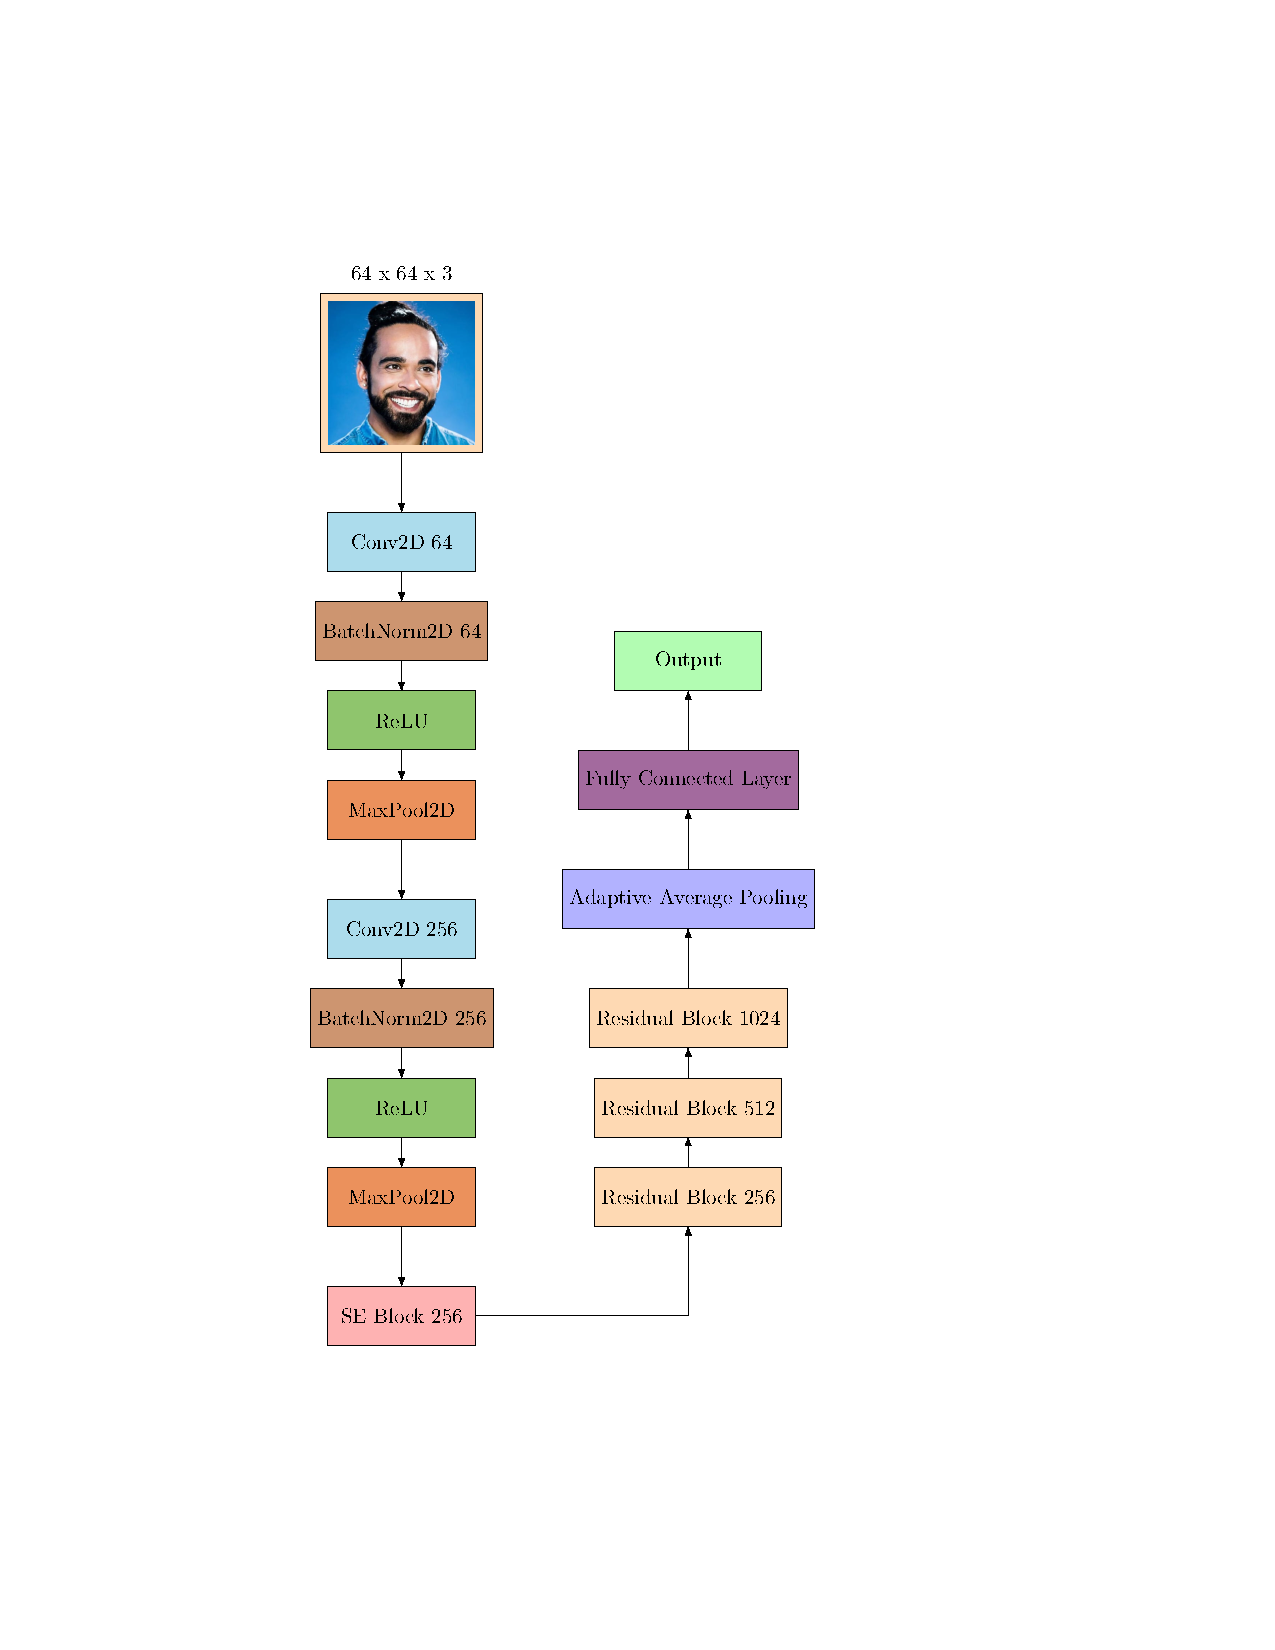
\includegraphics[width=0.7\textwidth]{Images/architecture}
	\caption{Model Architecture of the proposed FourForAll.}
	\Description{}{Here ``SE Block'' stands for Squeeze and Excitation Block. The method contains three steps. Firstly, the basic CNN block is applied to extract the basic features from facial images. Then, the SE block keeps the good features and suppresses the rest. In addition, the Residual blocks helps in extracting complex features from the feature map. Finally, a fully connected layer is employed to produce the classification result.}
\end{figure*}

\subsection{Overview}
Figure 1 illustrates the overall architecture of the proposed FourForAll. The proposed FourForAll is built upon a simple CNN block, combined with the squeeze and excitation block as well as residual blocks. Specially layers after the convolutional layer of block 3, the SE block and the residual blocks with the classifier are added to it.

Given an image sample, the input will go into the simple CNN block to support the feature-extracting capabilities of the model on the lower-level details of the image. The output feature maps are then used as input for the SE block, where meaningful features are kept and the rest are suppressed. The output feature maps from the SE block are then sent to the Residual blocks for meaningful local features are extracted. The output feature maps from the Residual blocks are in the dimensions of ${1 \times 1 \times  D}$, where $D$ represents the depth of the feature maps. The classifier takes the feature maps that have been adaptive average pooled as input, and outputs the probabilities of the facial expressions.

\subsection{Visual Geometry Group}
The Visual Geometry Group (VGG) model, created by Simonyan and Zisserman \cite{simonyan2014very} marks a significant advancement in the development of CNNs for tasks related to image recognition. Recognized for its uncomplicated design, the VGG utilizes a sequence of convolutional layers using compact ${3 \times 3}$ convolution filters, along with max-pooling layers, fully connected layers, and a softmax layer. This specific feature enables the VGG to grasp more intricate patterns by incorporating 16-19 weight layers in its architecture. We enhance VGG by incorporating batch normalization and dropout techniques to improve the stability of the learning process. Past research has demonstrated that the VGG model is efficient at categorizing extensive facial emotions, with its generalizability across different datasets leading to top-notch outcomes, underscoring the significance of depth in visual representations.

\subsection{Residual Network}
Training neural networks with increased parameters and deeper layers is generally more challenging. ResNet has become a revolutionary design, greatly improving performance in tasks like image classification, object detection, and semantic segmentation. ResNets use deep residual learning to achieve high accuracies on well-known datasets like ImageNet \cite{deng2009imagenet}. Taking inspiration from \cite{he2016deep}, we have incorporated ResNet18 and ResNet34 to simplify the training procedure. ResNet18 and ResNet34 are configurations of the ResNet architecture with 18 and 34 layers that tackle the vanishing/exploding gradient issue in training deep neural networks by using residual blocks. These residual blocks facilitate the direct flow of gradients in the network by incorporating the block's input with its output, allowing the training of even deeper networks than before.

\subsection{FourForAll}
The input for our emotion recognition model is an image with $3$ channels at ${64 \times 64}$ resolution. We implemented an emotion classifier from scratch with five convolution blocks as the baseline at the very beginning. Although a larger kernel is capable of offering a greater amount of information and a broader field of view because of additional parameters, we opt for a ${3 \times 3}$ kernel size in all convolutional layers, like the VGG model, because it is easier to train and does not require costly computations. After every convolutional layer, batch normalization is applied to stabilize the learning process by normalizing the input for each layer. Additionally, batch normalization guarantees that the variances of forward propagated signals are not zero.
